\documentclass{beamer}

\usepackage{beamerthemesplit}

\usepackage[utf8]{inputenc}
\usepackage[T1]{fontenc}
\usepackage{graphicx}
\usepackage{amsmath}
\usepackage{hyperref}
\usepackage{enumerate}

\title{Generating provable primes}
\author{Sigurd Meldgaard \and Kasper Damgård}
\date{7. Jan.}
\begin{document}
\maketitle

\begin{frame}
  \frametitle{Introduction} 

  \begin{itemize}
\item 
    Usually primes are generated by testing random numbers the
    randomized Miller-Rabin test 
\pause
\item If we know the factorization
    of $p-1$ where $p$ is prime, it is possible to generate a
    certificate showing the primality of $p$.  
\pause 
\item This way we
    can generate the prime ``bottom up'' in a recursive way.
    \pause
  \item We have implemented an algorithm constructing primes this way,
    and compared it to Miller-Rabin
  \end{itemize}
\end{frame}

\section{Theoretical background}
\begin{frame}
\frametitle{Euler's theorem}
\[
\forall n\in N, k, gcd(k,n)=1: k^{\phi(n)} \equiv 1 \mod n
\]
\end{frame}

\begin{frame}
\frametitle{Lucas' primality criterion}

Given a base $b$ and a prime candidate $n$. 

Where $gcd(b, n)=1$ and $b$ fulfills Fermat's equation for primes:
$b^{(n-1)}  \equiv  1    \mod n$

The smallest exponent where the sequence:
\[1, b^2, b^3 ... \mod n\]
reaches $1$ is called the period of $b$ mod $n$ or $ord_p(b)$. 

We know that 
\[b^{\phi(n)} \equiv 1 \mod n\]
 so 
\[ord_p(b)|\phi(n).\] 

\end{frame}
\begin{frame}
\frametitle{Lucas' primality criterion cont...}
We know that
\[ord_p(b)|\phi(n).\] 

And also that 
\[ord_p(b)|(n-1)\]

or equivalently $n-1 = x\cdot ord_p(b)$ for some positive integer $x$.

If we can prove $x=1$ then 
\[ord_p(b)=n-1=\phi(n)\] 
because: $\phi(n) \leq
n-1$, and then $n$ must be prime.
\end{frame}
\begin{frame}
\frametitle{Lucas' primality criterion cont...}
Assume we know the factorization of $n-1 = q_1^{\beta_1}q_2^{\beta_2}\ldots q_r^{\beta_r}$.

Then we can check that:
\[b^{(n-1)/q_i}\not\equiv 1 \mod n, i\in{1..r}\] If we raise $b$
to a power not a multiple of $ord_p(b)$ it will be different from $1$,
so $(n-1)/q_i\not|ord_p(b)$ for any $i$ 

And if that is true, all factors of $n-1$ are not factors of $x$, and
therefore $x=1$.

%. Because only primes have
%$\phi(n) = n-1$
\end{frame}
\begin{frame}
\frametitle{Using Lucas to generate primes}

\begin{itemize}
\item 
  For generating large primes we can recursively generate smaller
  primes, multiply them and see if the product plus one is a prime by
  testing for Lucas' criterion.
\pause
\item
  For the base case (primes smaller than a certain threshold) we use
  trial division of a random number to construct the prime.
\end{itemize}
\end{frame}
\begin{frame}
\frametitle{Let the half be random}
Really we only need to know the factorization of $F$ (if $F$ is odd),
generate $R$ randomly < $F$ and let:

\[n = 2RF+1\] 

Because if $F$
is odd and the test succeeds for some base $b$ the smallest possible
prime factor of $n$ is $2F+1$, and because $F>R$ $n=(2RF+1)<(2F+1)^2$,
$n$ must be prime.
\end{frame}
\begin{frame}
As explained in \cite{Mihailescu:1994:FGP} almost any base will work
for showing the primality of $p$, the exact proportion of good bases
is:

\[\phi(F)/F \geq 1-\sum^r_{j=1}1/q_j\]
\end{frame}
\begin{frame}
  \begin{itemize}
\item 
    To ensure that the primes are generated reasonably uniformly the
    size of the smaller primes generated in the recursive calls must
    be chosen properly.
\pause
\item
    In \cite{Mihailescu:1994:FGP} a method is given for choosing the
    sizes from the distribution of the relative size of the largest
    factor of a random integer $F$. And it is argued that the
    conditional distribution given that $2F+1$ is prime is almost the
    same.
\pause
\item
    Also it is noted that if $F$ has only one prime factor, we still
    choose from among 10 \% of all primes.
    
  \end{itemize}
\end{frame}
\begin{frame}
  \frametitle{Asymptotic running time}
The asymptotic estimated running time of finding a $k$-bit prime with the
asymptotically best multi-precision algorithms is:
\[O(k^3\cdot\log\log(k)).\]
For straightforward integer arithmetic the estimated running time is:
\[O(\frac{k^{4}}{\log(k)})\]
\end{frame}
\section{The algorithm}
\begin{frame}
\frametitle{The base case}
\noindent
$\text{PROVABLE PRIME}(k)$\\
INPUT: a positive integer $k$.\\
OUTPUT: a $k$-bit prime number $n$.
\begin{enumerate}
\item (If $k$ is small, then test random integers by trial division. A table of small primes may 
be precomputed for this purpose.) 
If $k \leq 20$ then repeatedly do the following: 
\begin{enumerate}
\item Select a random $k$-bit odd integer n. 
\item Use trial division by all primes less than $\sqrt{n}$ to determine whether $n$ is prime. 
\item If $n$ is prime then return(n).
\end{enumerate}
\end{enumerate}
\end{frame}
\begin{frame}
\frametitle{The recursive case}
\begin{enumerate}

  \setcounter{enumi}{1}
\item Set $c\leftarrow 0.1$ and $m\leftarrow 20$. 
\item (Trial division bound) Set $B\leftarrow c \cdot k^2$. 
\item (Generate r, the size of q relative to n) If k > 2m then repeatedly 
do the following: select a random number s in the interval [0, 1], set $r\leftarrow 2^{s-1}$ , until 
$(k - rk) > m$. Otherwise (i.e. $k \leq 2m$), set $r\leftarrow 0.5$. 
\item Compute $q\leftarrow \text{PROVABLE PRIME}(\lfloor r \cdot k \rfloor + 1)$. 
\item Set $I \leftarrow \lfloor 2^{k-1} /(2q) \rfloor$.
\end{enumerate} 
\end{frame}

\begin{frame}
\frametitle{The recursive case 2 (testing candidates)}
\begin{enumerate}
  \setcounter{enumi}{6}
\item $success\leftarrow False$. 
\item While (not $success$) do the following:
  \begin{enumerate}
\item (select a candidate integer $n$) Select a random integer $R$ in the interval 
$[I + 1, 2I]$ and set $n\leftarrow 2Rq + 1$. 
\item Select a random integer a in the interval $[2, n - 2]$. 

Compute $b\leftarrow a^{n-1} \mod n$. 

If $b = 1$ do the following: 

\ \ \ Compute $b\leftarrow a^{2R} \mod n$ and $d\leftarrow  gcd(b - 1, n)$.

\ \ \ If $d = 1$ then $success\leftarrow True$.
\end{enumerate} 
\item Return(n). 
\end{enumerate}
\end{frame}

\section{Implementation}
\begin{frame}
\frametitle{Optimizations}
\begin{itemize}
\item Do a single Miller-Rabin test with base 2 of $2FR+1$ before
  actually testing for Lucas' primality criterion.

  Quickly weeds out most of the composites.
\end{itemize}
\end{frame}

\begin{frame}
Implemented the algorithm in Python.
\begin{itemize}
\item Used the built-in multi-precision integers.

\item Speed loss due to interpretation is negligible. (Most time is
  spent doing exponentiations)


\item We also implemented the Miller-Rabin primality test for
  comparison.
\end{itemize}
\end{frame}

\section{Results}
\begin{frame}
  \begin{itemize}
  \item There are big deviations from the average, this is due to the
    algorithm depending a lot on ``being lucky'' when choosing the
    random parameters.

  \item For practical purposes one would want to do the Miller-Rabin
    test for several bases to make the probability of accepting a
    composite number negligibly small.
  \end{itemize}
\end{frame}

\begin{frame}
\begin{figure}[h]
  \centering
  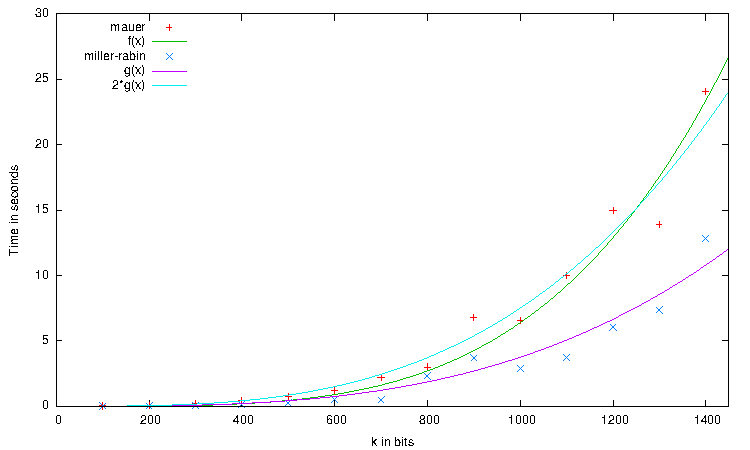
\includegraphics[scale=0.8]{plot.pdf}
  \caption{Timings of the two prime construction methods}
  \label{fig:timings}
\end{figure}
\end{frame}

\section{Conclusion}
\begin{frame}
  \frametitle{Conclusion}
Generating provable primes for public key parameters is certainly
practically possible. But Miller-Rabin test is easier to implement and
can construct pseudoprimes with very high certainty in ca. the same
time. And these numbers will be distributed truly uniformly among all
primes.
\end{frame}

\end{document}
